\documentclass[12pt, a4paper, twoside]{book}
\usepackage[utf8]{inputenc} % Aceptar diferentes tipos de codificación de caracteres de entrada (en este caso usamos la codificación Unicode UTF-8)
%\usepackage{natbib}
\usepackage{listings}
\usepackage{eurosym}
\usepackage[spanish]{babel}
\usepackage{titlesec}
\usepackage{graphicx} % Soporte aumentado para gráficos 
\usepackage{float}
\usepackage{hyperref} % Para manejar referencias cruzadas. P.ej. añadir hiperenlaces al índice
\usepackage{caption}
\usepackage{setspace}
\usepackage{color}
\usepackage[a4paper, top=3.5cm, bottom=3.5cm, left=3cm, right=3cm]{geometry}
\spacing{1.5}
\setcounter{secnumdepth}{4}
\setlength{\parindent}{12pt}
\titleformat{\paragraph}
{\normalfont\normalsize\bfseries}{\theparagraph}{1em}{}
\titlespacing*{\paragraph}
{0pt}{3.25ex plus 1ex minus .2ex}{1.5ex plus .2ex}

%\usepackage{inconsolata}
%
%\usepackage[T1]{fontenc}
%
%\definecolor{pblue}{rgb}{0.13,0.13,1}
%\definecolor{pgreen}{rgb}{0,0.5,0}
%\definecolor{pred}{rgb}{0.9,0,0}
%\definecolor{pgrey}{rgb}{0.46,0.45,0.48}
%
%\lstset{language=Java,
%	showspaces=false,
%	showtabs=false,
%	breaklines=true,
%	showstringspaces=false,
%	breakatwhitespace=true,
%	commentstyle=\color{pgreen},
%	keywordstyle=\color{pblue},
%	stringstyle=\color{pred},
%	basicstyle=\ttfamily,
%	moredelim=[il][\textcolor{pgrey}]{$$},
%	moredelim=[is][\textolor{pgrey}]{\%\%}{\%%}
%}


\begin{document}	
	
	\thispagestyle{empty} 	
	%%%%%%%%%%%%%%%%%%%%%%%%%%%%%%%%%%%%%%%%%%%%%%%%%%%%%%%%%%%%%%%%%%%%%%%%%%%%%%%%
	% PORTADA
	%%%%%%%%%%%%%%%%%%%%%%%%%%%%%%%%%%%%%%%%%%%%%%%%%%%%%%%%%%%%%%%%%%%%%%%%%%%%%%%%
	
	\begin{center}		
		
\includegraphics[width=15cm]{Imagenes/Simbolo_logo_UDC.png}
	\end{center}
	
	% Lista de tamaños: \Huge, \huge, \LARGE, \Large, \large, \small, \footnotesize, \tiny
	\vspace{2cm}
	
	\begin{center}		
		{\textbf{ FACULTADE DE INFORMÁTICA}}
			
		\vspace{1cm}
		\LARGE{ TRABALLO FIN DE MÁSTER }	\\
		\LARGE{ MÁSTER UNIVERSITARIO EN INGENIERÍA INFORMÁTICA } \\
		\vspace{1cm}	
		\LARGE{\textbf{ Aplicación web para a xestión de menús domésticos con servizos nutricionais : Eat Fit Week! }}
	\end{center}
	
	\vspace{2cm}
	\hfill \textbf{Autor: \textit{Elías Ferreiro Borreiros}}
	
	
	\hfill \textbf{Director: \textit{Juan José Sánchez Penas}} 
	
	
	\hfill A Coruña, Agosto, 2019					
	
	
	\clearpage
	
	\vspace*{\fill}
	\hfill A mi familia
	\vspace*{\fill}
	
	
	\clearpage
	
	\begin{center}
		\LARGE{\textbf{ AGRADECIMIENTOS }}	
	\end{center}	
	A mi familia y a mis amigos, por su apoyo incondicional y su paciencia.\\
	A Esther por estar ahí para mí incluso en los días más duros o sobre todo en ellos.
	
	\clearpage
	
	\begin{center}
		\LARGE{\textbf{ RESUMEN }}	
	\end{center}
	Hoy en día, con el cambio en los estilos de vida de las personas y tendiendo hacia unas costumbres más sedentarias, hay una mayor necesidad de enfocarse en una dieta equilibrada y saludable.
	Para ello, se han desarrollado muchos sistemas webs y móviles para la gestión de comidas y de sus valores nutricionales.	Sin embargo, analizando esos sistemas, vemos que tienen un error en su planteamiento al inundar a los usuarios con formularios sobrecargados y repletos de información innecesaria. 
	El otro problema principal de estos sistemas es la cantidad exagerada de trabajo manual que debe hacer el usuario antes de poder disfrutar de la funcionalidad principal. 

	Para resolver todo esto, hemos decidido plantear el desarrollo de una aplicación que solvente estos problemas y ofrezca una funcionalidad que no disponen los competidores : el análisis nutricional dinámico de las comidas planificadas para la semana configurable por el usuario.
	El usuario dispondrá de unos ciertos parámetros para la planificación de sus menús: cantidad de calorías, proteínas, grasas ...
	Una vez configurados, a medida que se vayan añadiendo platos al menú semanal se verificarán estos parámetros para indicar al usuario si está cumpliendo con sus especificaciones o si se está sobrepasando.

	A mayores permitiremos la gestión de las entidades necesarias para esta planificación: ingredientes, platos, menús ... 
	Esto se hará siguiendo la filosofía inicial del proyecto: simplificar la entrada lo más posible y disminuir el esfuerzo requerido por el usuario. 
	Para esto llamaremos a servicios externos que nos permitirán estimar las características nutricionales de los ingredientes de forma que el usuario no tendrá que indicar esos datos y permitiremos con cada registro de usuario el alta automática de unos ingredientes base utilizables en la mayoría de recetas que agilizarán la configuración necesaria de un nuevo perfil para permitir disfrutar al máximo al usuario de las funcionalidades realmente importantes desde el momento más temprano posible.
	
	\clearpage
	
	\textbf{Título:} Aplicación web para a xestión de menús domésticos con servizos nutricionais
	\\
	\textbf{Autor:} Elías Ferreiro Borreiros
	\\
	\textbf{Tutor/Director:} Juan José Sánchez Penas
	
	
	\textbf{Palabras clave:} Java EE, POJO, Maven, Angular JS, Spring, Hibernate, Web, MySQL, Tarea, Lista, Contexto, Cliente - Servidor, Food, Planning, Management, Scrum. 
	
	
	\renewcommand{\contentsname}{Índice de contenidos}
	\renewcommand{\listfigurename}{Índice de figuras}
	\renewcommand{\listtablename}{Índice de tablas}
	
	\tableofcontents % indice de contenidos
	
	\listoffigures % indice de figuras
	
	\listoftables % indice de tablas
	
	\clearpage
	
	\chapter{Motivación}	
	\chapter{Fundamentos teóricos}
	\chapter{Determinación de la situación actual}
	\chapter{BASE TECNÓLOGICA}
	\section{Lenguajes}
	\subsection{Java SE 8}
	\subsection{HTML}
	\subsection{CSS}
	\section{Frameworks y librerías}
	\subsection{Core}
	\subsubsection{Spring}
	\subsubsection{Hibernate}	
	\section{Web}
	\subsubsection{Angular JS}
	\subsubsection{Bootstrap}     
	\subsection{Pruebas}
	\subsubsection{JUnit}
	\subsubsection{Spring Test Context}
	\subsubsection{Eclemma}	
	\subsection{Protocolos}
	\section{Hypertext Transfer Protocol o HTTP}
	\subsection{Herramientas de Desarrollo}
	\section{Maven}
	\subsection{Servidores de Aplicaciones}
	\subsection{Sistemas de Gestión de Bases de Datos}
	\subsection{Herramientas de apoyo}
	\chapter{INTRODUCCIÓN AL DESARROLLO REALIZADO}
	\section{Introducción}
	\section{Tecnologías}
	\section{Metodología e Iteraciones}
	\subsection{Proceso Unificado}
	\subsubsection{Fases del proceso unificado}
	\subsubsection{Fase de Inicio}
	\subsection{Iteraciones}
	\chapter{PLANIFICACIÓN Y ANÁLISIS DE COSTES}
	\section{Análisis de viabilidad}
	\section{Planificación}
	\subsection{Planificación previa}
	\subsection{Iteraciones}
	\subsection{Diagrama de Gantt}

	\chapter{REQUISITOS DEL SISTEMA}
	\section{Introducción}
	\section{Actores}
	\section{Casos de Uso}
	\subsection{Casos de uso comunes}		 
	\section{Modelo de Casos de uso}
	\subsection{Casos de uso comunes}
	\subsection{Casos de uso usuario}
	\subsection{Casos de uso administrador}
	\chapter{DISEÑO DE LA APLICACIÓN}
	\section{Introducción y Objetivos}
	
	\section{Arquitectura general}
	
	El sistema se divide en dos subsistemas principales : efw-back y efw-front.
	
	\section{Subsistema Backend efw-back}
	
	El backend del sistema está desarrollado como una serie de APIs REST totalmente aisladas del frontal de forma que sean independientes del mismo y puedan utilizarse por cualquier otro posible frontal que se requiera en el futuro (Aplicaciones nativas móviles, por ejemplo).
	
	\subsection{Arquitectura}
	
	La arquitectura del backend se compone de cuatro elementos principales :
	
	\begin{itemize}
		\item Controladores REST que reciben cada una de las peticiones que realizará el frontal y se encargarán de validar que los parámetros de entradas de cada una de ellas se encuentran en el formato correcto con los datos necesarios y, en caso de no estarlo, pararán la petición devolverán un código y mensaje de error identificativos.
		\item Servicios, los principales contenedores de la lógica de negocio. Son invocados por los controladores y ellos a su vez invocan a los diferentes repositorios de acceso a datos para obtener la información necesaria para cada petición concreta. Preparan esta información en el formato necesario de la respuesta en caso de una petición de consulta o bien utilizarán los datos recibidos para hacer las actualizaciones correspondientes a una petición de actualización / modificación / borrado / inserciones.
		\item Repositorios, los encargados de las ejecuciones de las consultas / actualizaciones / borrados / inserciones sobre las propias bases de datos siguiendo las entidades configuradas.
		\item Entidades de base de datos de hibernate, cada una correspondiente a una tabla. Definen las columnas de su tabla correspondiente así como sus relaciones entre ellas.
	\end{itemize} 
	
	\subsection{Modelo del dominio}    
	\subsubsection{Diagrama de Entidades}
	En la figura se muestra el diagrama de entidades de la aplicación.
	\begin{figure}[H]
		\centering
		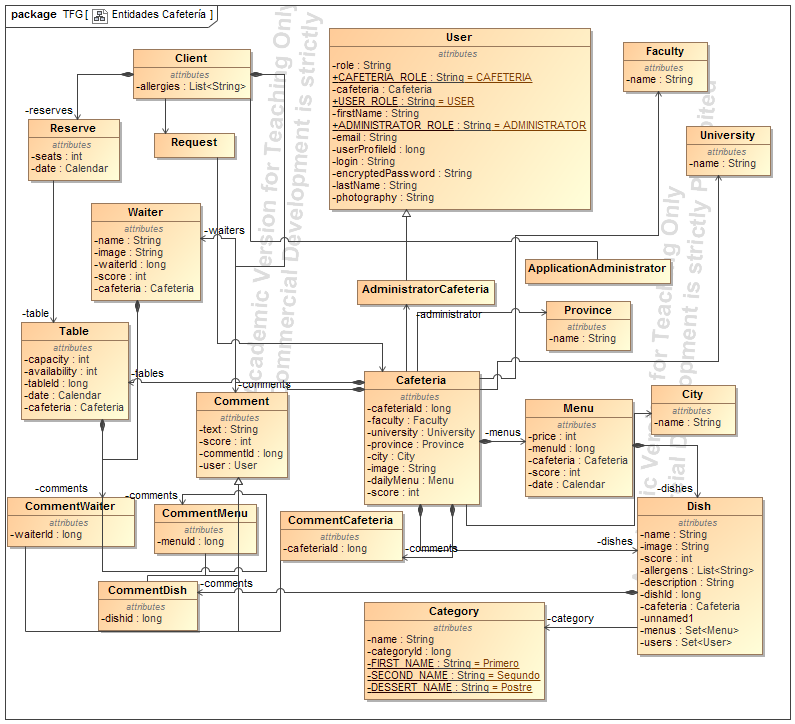
\includegraphics[width=15cm]{Imagenes/DiagramaClases.png}
		\caption{Diagrama de clases}\label{Diagrama de clases}
	\end{figure}
	\subsubsection{Modelo de Datos}
	A continuación se describirán todas las entidades principales de la aplicación.
	\begin{itemize}
		\item Descripción de entidades
		\begin{itemize}
			\item User \\Entidad representante de las personas que accederán a la misma. Es la entidad propietaria del resto de forma que puede tener Ingredientes, Platos, Menus ... asignados. Puede configurar gran parte de su funcionalidad en la aplicación mediante configuraciones de usuario.
			\item UserConfiguration \\ Cada una de las configuraciones de usuario que le permiten personalizar el funcionamiento del sistema para él en concreto como pueden ser : la cantidad de calorías por semana que se auto permite, las comidas al día que realiza y sus nombre ...
			\item Meal \\ Cada una de las comidas que se configura el usuario que le aparecen en sus calendarios y que puede permitir o restringir de sus platos. Tienen una hora asignada cada una de ellas para poder ordenarlas en la visualización de los calendarios.
			\item Ingredient \\ Cada uno de los ingredientes registrados por el usuario para su combinación en platos. Registran su nombre y sus stats nutricionales : calorías, proteinas, grasas y carbohidratos. Pueden pertenecer a una categoría alimenticia
			\item FoodCategory \\ Cada una de las categorías alimenticias a las que pueden pertenecer los ingredientes del usuario. Pueden ser prohibidas por el usuario para recordarse de que debe tener cuidado con esos ingredientes concretos.
			\item Dish \\ Cada uno de los platos que registra el usuario juntando de uno a varios ingredientes con una cantidad concreta y permitiendo especificar una receta de elaboración. Tienen stats nutricionales calculados como la suma de los stats de sus ingredientes en relación a su cantidad en el plato.
			\item Menu \\ Cada uno de los menú semanales que planifica el usuario del sistema. Están formados por un conjunto de platos asignados a una fecha concreta. Tienen stats nutricionales calculados como la suma de los stats de sus platos. Permiten obtener los elementos de su lista de la compra correspondiente como los ingredientes necesarios para todos sus platos con las unidades y la cantidad necesaria de cada uno.
		\end{itemize}
		\item Descripción de relaciones
		\begin{itemize}
			\item Relación Dish - Meal: Dispone de una relación N:M ya que un plato puede estar permitido en varias comidas del usuario y una comida tendrá varios platos permitidos.
			\item Relación Dish - Ingredient: Dispone de una relación N:M ya que un plato puede tener varios ingredientes y un mismo ingrediente puede aparecer en varios platos. Como atributo de la relación tenemos la cantidad que tendrá el ingredient en el plato concreto.
			\item Relación Dish - User: Dispone de una relación N:M ya que un plato puede aparecer en varios usuarios y un usuario puede tener varios platos.
			\item Relación Dish - Menu: Dispone de una relación N:M ya que un plato puede aparecer en varios menús y un menú tendrá por naturaleza varios platos. Como atributo de la relación tenemos la fecha concreta en la que el plato está registrado en el menú.
			\item Relación Ingredient - FoodCategory: Dispone de una relación 1:N ya que un ingrediente solo pertenecerá a una categoría pero una categoría tendrá varios ingredientes.
			\item Relación Ingredient - User: Dispone de una relación N:M ya que un ingrediente puede pertenecer a varios usuarios y un usuario puede tener varios ingredientes registrados.
			\item Relación User - Meal: Dispone de una relación 1:N ya que un usuario puede tener varias comidas registradas pero cada comida solo estará asignada a un usuario concreto.
			\item Relación User - UserConfiguration: Dispone de una relación 1:N ya que un usuario puede tener varias configuraciones pero cada configuración pertenecerá a un único usuario.
			\item Relación User - Menu: Dispone de una relación 1:N ya que un usuario puede tener varios menús registrados pero cada menú pertenecerá a un único usuario.
			\item Relación User - MenuTemplate: Dispone de una relación 1:N ya que un usuario puede tener varias plantillas de menú pero cada plantilla tendrá un único usuario.
			\item Relación Menu - MenuTemplate: Dispone de una relación 1:N ya que un menú puede generar varias plantillas pero cada plantilla pertenece a un único menú.
		\end{itemize}
	\end{itemize}	
	\subsubsection{Diagrama de Entidad Relación}
	A continuación, mostramos el diagrama entidad relación de base de datos empleado para la definición de las tablas, sus atributos y sus relaciones.
	\begin{figure}[H]
		\centering
		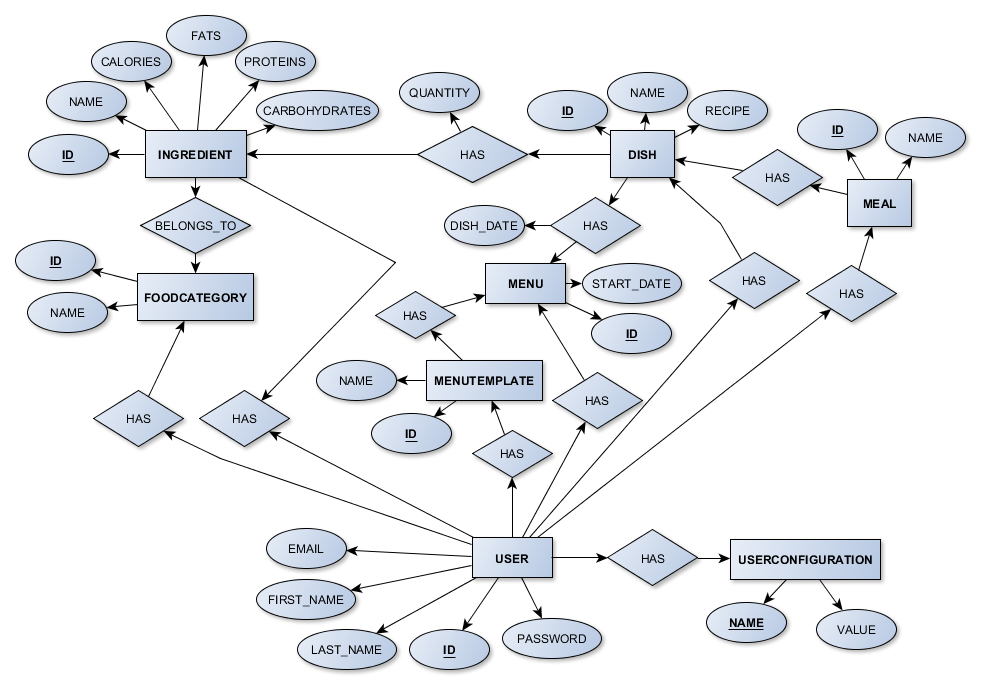
\includegraphics[width=15cm]{Imagenes/EntidadRelacion.png}
		\caption{Entidad relacion}\label{Entidad relacion}
	\end{figure}
	
	\subsection{Capa de Acceso a Datos}
	
	Empleamos repositorios implementados mediante Spring Data con lo que las consultas se infieren del nombre de los métodos a través de los atributos de la entidad de Hibernate utilizada en el repositorio concreto.
	
	Todos estos repositorios presentan métodos básicos de CRUD sobre su entidad correspondiente : 
	\begin{itemize}
		\item void delete(Entity e) -> Elimina la entidad pasada como parámetro.
		\item List<Entity> findAll() -> Obtiene todas las filas de esa entidad de base de datos sin ningún filtro aplicado.
		\item Entity findOne(int id) -> Obtiene una fila concreta de la entidad correspondiente con el id único pasado como parámetro.
		\item Entity save(Entity e) -> Inserta la entidad pasada como parámetro, o bien la actualiza en caso de ya existir previamente, con los datos guardados en el objeto del parámetro.
	\end{itemize}
	
	La aplicación presenta los siguientes repositorios:
	
	\begin{itemize}
		\item UserRepository: Además de las operaciones básicas de todos los repositorios dispone de un método de búsqueda de usuarios por email para el proceso de login de un usuario concreto a través de su email y contraseña.
		\item UserConfigurationRepository: Además de las operaciones básicas, dispone de un método de búsqueda de configuraciones de usuario por nombre de la configuración y el id del usuario al que se le quieren consultar las configuraciones.
		\item MenuTemplateRepository: Además de las operaciones básicas, dispone de un método de búsqueda de plantillas de menús para un usuario concreto.
		\item MenuRepository: Además de las operaciones básicas, dispone de un método de búsqueda de un menú a través de su id de usuario y de su fecha inicial.
		\item MenuDisRelRepository: Utilizado para dos operaciones de borrado concretas: Borrado por id de menú utilizado en la funcionalidad de limpiado de menú y borrado por ids (id de menú, fecha e id de plato) para las funcionalidades de borrado de plato de menú y la funcionalidad de actualización de fecha de plato en menú.
		\item MealRepository: Además de las operaciones básicas, dispone de una búsqueda por id de usuario ordenada por hora de la comida.
		\item IngredientRepository: Dispone de tres consultas custom : búsqueda de ingredientes por usuario para su visualización, búsqueda por usuario y nombre para verificar la unicidad del nombre de ingredientes en la inserción, búsqueda de otros ingredientes del usuario con mismo nombre para verificar la unicidad de nombre en la actualización
		\item FoodCategoryRepository: Dispone de una consulta custom para encontrar categorías que cumplan una lista de ids concretos para visualizar las categorías que el usuario tiene configuradas como prohibidas.
		\item DishRepository: Dispone de tres consultas custom : búsqueda de platos por usuario para su visualización, búsqueda por usuario y nombre para verificar la unicidad del nombre de platos en la inserción, búsqueda de otros platos del usuario con mismo nombre para verificar la unicidad de nombre en la actualización
		\item CustomQueryRepository: Disponemos de un repositorio concreto utilizado para una consulta concreta necesaria para la funcionalidad de Machine Learning cuya complejidad es demasiado grande para poder realizarla de forma eficiente con Spring Data. Para un usuario, obtiene de todos sus menús los tres valores siguientes : Día de la semana - Nombre de comida - Plato asignado a ese hueco. 	
	\end{itemize}
	
	\subsection{Capa Servicios del Modelo}
	Como comentábamos en el principio del subsistema backend, tenemos una serie de servicios de negocio para dar soporte a cada una de las peticiones REST permitidas. 
	Para cada uno de ellos se define una interfaz en la que se indican todos los métodos del servicio y su firma. Tenemos por otro lado una clase que implementa esta interfaz y todos sus métodos.
	\begin{itemize}
		\item DishService : 
		\begin{itemize}
			\item create: Servicio utilizado para crear nuevos platos. Se le indica el usuario para el que se quiere registrar, el nombre del plato, la receta, sus ingredientes y cada una de sus cantidades así como las comidas en las que el plato debe estar permitido. Lo primero que se verifica es que el usuario no tenga ya un plato con este nombre en cuyo caso se devolvería un error indicándolo. En caso contrario, se registra el plato con los datos informados.
			\item delete: Servicio utilizado para eliminar platos existentes por id. Se consulta el plato correspondiente al id informado. En caso de no existir, se devuelve un error indicándolo. En caso contrario se elimina el plato a través del repositorio.
			\item findUserDishes: Servicio utilizado para obtener todos los platos de un usuario a través del id del usuario. Los platos obtenidos se transforman para ceñirse al formato de respuesta de la petición: id de plato, nombre, receta, ingredientes y sus cantidades, comidas permitidas y lista de stats nutricionales del plato calculados como la suma de los de sus ingredientes en relación a su cantidad en el plato.
			\item update: Servicio utilizado para actualizar un plato existente. Se comprueba que existe un plato con el id indicado, en caso de no ser así se devuelve un error informativo. En caso de existir, se comprueba que el nuevo nombre a establecer no esté siendo usado por otro plato del usuario. En caso de no cambiar el nombre o bien de estar libre el nuevo nombre se actualiza la información indicada en el plato.
		\end{itemize}
		\item IngredientService : 
		\begin{itemize}
			\item create: Servicio utilizado para crear nuevos ingredientes. Se le indica el usuario para el que se quiere registrar, el nombre del ingrediente y sus stats: calorías, proteinas, grasas y carbohidratos. Lo primero que se verifica es que el usuario no tenga ya un ingrediente con este nombre en cuyo caso se devolvería un error indicándolo. En caso contrario, se registra el ingrediente con los datos informados.
			\item delete: Servicio utilizado para eliminar ingredientes existentes por id. Se consulta el ingrediente correspondiente al id informado. En caso de no existir, se devuelve un error indicándolo. En caso contrario se elimina el ingrediente a través del repositorio.
			\item findUserIngredients: Servicio utilizado para obtener todos los ingredientes de un usuario a través del id del usuario. Los ingredientes obtenidos se transforman para ceñirse al formato de respuesta de la petición: id de ingrediente, nombre, categoria alimenticia(id y nombre) y lista de stats nutricionales del ingrediente.
			\item update: Servicio utilizado para actualizar un ingrediente existente. Se comprueba que existe un ingrediente con el id indicado, en caso de no ser así se devuelve un error informativo. En caso de existir, se comprueba que el nuevo nombre a establecer no esté siendo usado por otro plato del usuario. En caso de no cambiar el nombre o bien de estar libre el nuevo nombre se actualiza la información indicada en el ingrediente.
			\item getNutritionEstimate: Servicio de obtención de los stats nutricionales de un ingrediente a través de su nombre. Se delega en el servicio rest externo de estimación de stats nutricionales por ingrediente para estimarlos a través del nombre de ingrediente recibido como parámetro. Se transforman los stats recibidos con la cantidad de ingrediente recibida para transformarlos de forma que se muestren "/ 100 gramos".
			\item getFoodCategories: Servicio de obtención de todas las categorías alimenticias delegando la consulta en el repositorio de categorías alimenticias.
		\end{itemize}
		\item MachineLearningService : 
		\begin{itemize}
			\item evaluateInstance: Servicio utilizado para, a través de Weka, predecir el nombre del plato predicho para un Día de Semana y una Comida concreta. El servicio recibe la lista de todas las combinaciones registradas de {Día de semana, Comida, Nombre de plato} de ese usuario hasta el momento. Con estos datos se entrena la el clasificador para que pueda predecir la nueva instancia solicitada. Se devuelve la predicción en forma de nombre de plato.
		\end{itemize}
		\item MenuService :
		\begin{itemize}
			\item create: Servicio utilizado para crear nuevos menús. Se le indica el usuario para el que se quiere registrar y la fecha de inicio del menú a crear. La fecha recibida puede corresponderse con cualquier de la semana con lo que, a partir de ella, obtenemos el inicio de semana más cercano hacia atrás en el tiempo (En caso de recibirse un domingo 25 se obtiene el lunes 19 por ejemplo). Este lunes se establece en el menú a crear y se crea a través del repositorio de menús.
			\item clearMenu: Servicio utilizado para limpiar el menú de platos a través del id del menú. En caso de no encontrarse un menú con este id se devuelve un error indicativo. En caso de encontrarse, se borran todas las relaciones entre este menú y sus platos de forma que el menú queda vacío.
			\item findUserMenu: Servicio utilizado para obtener el menú de un usuario en una fecha dada. A través de la fecha recibida se obtiene el inicio de semana más cercano como se hace en la creación de menús.
			\item addDishToMenu: Servicio utilizado para añadir un plato a un menú. Se reciben el id del menú, el id del plato y la fecha en la que se quiere añadir. Se buscan el menú y el plato por los ids, en caso de no encotnrarlos, se devuelve un error significativo. En caso contrario se registra la nueva relación entre el menú y el plato en la fecha correspondiente.
			\item addDishToFirstValidSpotOnMenu: Servicio uilizado para añadir un plato al hueco válido más temprano posible de un menú. Se reciben el id del usuario al que pertenece el menú así como el id del plato que se quiere añadir. Primero, se obtiene el menú actual del usuario a través del id de usuario y el inicio de semana correspondiente al día actual. A continuación se busca el hueco disponible más cercano para el menú y el plato, la fecha más cercana con una comida permitida por el plato.
			\item updateDishDateOnMenu: Servicio utilizado para actualizar la fecha de un plato en un menú. Se reciben el id del menú, el id del plato, la fecha actual en el menú y la fecha nueva que se desea. A través de estos datos se obtiene la relación entre el plato y el menú, se elimina y se monta la nueva relación con la nueva fecha.
			\item removeDishFromMenu: Servicio utilizado para eliminar la relación de un plato y un menú en una fecha concreta. Se reciben el id del menú, el id del plato y la fecha de la relación que se quiere eliminar. Se obtiene la relación a través de estos datos y se elimina.
			\item getShoppingList: Servicio utilizado para obtener la lista de la compra de un menú. Se recibe el id del menú. A través del menú, se obtienen los ingredientes de cada uno de sus platos, se agrupan y se obtiene tanto el número de veces que aparece cada ingrediente como la cantidad total en gramos de los ingredientes. En este método se delega en el servicio de estimación de precio de mercadona que utiliza los datos scrappeados del catálogo de mercadona para sacar una estimación del precio total de la lista de la compra generada.
			\item randomGenerateMenu: Servicio utilizado para rellenar un menú con los platos del usuario aleatoriamente. Se recibe el id del menú, en caso de no estar ya vacío, se limpia de platos el menú y a continuación se rellena aleatoriamente con los platos del usuario. Se itera por los días del menú y en cada comida del día se selecciona aleatoriamente un plato de entre los platos del usuario que tienen permitida esa comida.
			\item generateValidMenu: Servicio utilizado para rellenar un menú de forma que no se incumplan los límites de stats del usuario. Se recibe el id del menú, en caso de no estar ya vacío, se limpia de platos el menú y a continuación se rellena válidamente con los platos del usuario. Se itera por los días del menú y en cada comida del día se selecciona un plato válido para ese hueco : que tenga esa comida permitida y cuyos stats más los que tenemos por el momento en el menú no incumplan algunos de los límites del usuario. En caso de no poder seleccionar ningún plato, se para la generación del menú y se deja rellenado hasta lo máximo que podemos.
			\item fillMenuFromTemplate: Servicio utilizado para rellenar un menú a través de una plantilla. Se reciben el id del menú a rellenar y el id de la plantilla a aplicar. Se consulta el menú a rellenar, en caso de no estar ya vacío, se vacía de platos y se rellena con los platos registrados en la plantilla en los huecos correspondientes en el nuevo menú.
			\item machineLearningSuggestDish: Servicio utilizado para predecir el Plato correcto para un hueco de menú en función de los gustos del usuario. Se reciben el id del menú y la fecha en la que se quiere obtener el plato sugerido. Se delega en el repositorio de queries custom para obtener para el usuario todas las tuplas {Día de semana, Comida, Nombre de plato} de los menús registrados en el sistema del usuario. Se delega en el servicio de machine learning para obtener el plato sugerido en función de estos datos y, en caso de obtenerse un plato, se agrega al menú en el hueco indicado.
		\end{itemize}
		\item MenuTemplateService :
		\begin{itemize}
			\item saveMenuAsTemplate: Servicio utilizado para generar una plantilla a través de un menú. Se reciben el id del menu que se quiere utilizar para generar la plantilla, el nombre que se le quiere asignar y el menú en el que inspirar la plantilla. Se obtiene el menu y el usuario a traves de sus ids y se genera la nueva plantilla a través de los platos del menú obtenido y se registra en el usuario.
		\end{itemize}
		\item MercadonaPriceEstimateService : 
		\begin{itemize}
			\item estimateShoppingList: Servicio utilizado para estimar el precio de una lista de la compra en función de los precios de mercadona. Se reciben los elementos de la lista de la compra y sus unidades. Se procesa el excel obtenido a través de los scrapeos de la página web de mercadona, se buscan los elementos de la lista de la compra en este excel y se accede a sus precios.
		\end{itemize}
		\item UserConfigurationService :
		\begin{itemize}
			\item findUserConfigurationByNameOrDefault: Servicio utilizado para obtener el valor de una configuración de usuario por nombre e id de usuario. Se reciben el id de usuario, el nombre de la configuración, la clase a la que se debe castear el valor de la configuración y un valor por defecto que se devolverá en caso de no encontrarse la configuración consultada.
			\item findUserConfigurationListByNameOrDefault: Servicio utilizado para obtener el valor de una configuración de usuario en forma de lista. Se parseará el valor de la configuración con la clase indicada y se dividirá el valor de la configuración en elementos de la lista a devolver separados en el valor por ","
		\end{itemize}
		\item UserDataLoadService : Servicio utilizado para obtener los datos por defecto que se cargarán en un usuario al registrarlo por primera vez en el sistema.
		\begin{itemize}
			\item getDefaultMeals: Método utilizado para obtener las comidas por defecto que se cargan en nuevos usuarios. Tienen los valores : Desayuno, Comida y Cena.
		\end{itemize}
		\item UserService: 
		\begin{itemize}
			\item create: Método utilizado para registrar un nuevo usuario en el sistema. Recibe un nombre, un apellido, un email y una constraseña que se registrarán en el nuevo usuario. Se delega en el servicio de userDataLoad para cargar los datos por defecto de nuevos usuarios.
			\item updateUserConfigurations: Método utilizado para cambiar los valores de las configuraciones de usuario indicadas. Se reciben el id de usuario cuyas configuraciones cambian y los nuevos valores a cargar en ellas.
			\item findConfigurations: Método utilizado para obtener los valores de las configuraciones de usuario de un usuario concreto. Se recibe el id del usuario a consultar, se consultan sus configuraciones y se formatean para poder devolverlas con nombres y tipos concretos.
			\item login: Método utilizado para iniciar sesión con un usuario concreto. Se reciben un email y una contraseña que intentan iniciar sesión en el sistema. Se comprueba si se corresponden con los de algún usuario y en caso de corresponderse se devuelve login correcto. En otro caso se devuelve el error concreto.
		\end{itemize}
	\end{itemize}
	
	\section{Subsistema Frontend efw-front}
	
	El frontal Web desarrollado utiliza Angular JS y su arquitectura se centra en módulos y su subdivisión en componentes.
	
	Cada componente presenta los siguientes elementos : 
	\begin{itemize}
		\item Hoja de estilos CSS -> Los estilos necesarios para el html que forma el componente
		\item Plantilla HTML -> Los elementos que conforman la visualización del componente
		\item Controlador Typescript -> El controlador de los elementos definidos en la plantilla html. Contiene el servicio encargado de los datos. El propio controlador se centra en la gestión de las visualizaciones del componente.
		\item Servicio Typescript -> Contenedor de los cálculos de datos realizados en el frontal. Son también los responsables de las llamadas rest a los servicios expuestos por el backend.
	\end{itemize}

	\subsection{Módulos empleados}
	
	Se definen los siguientes módulos agrupados por dominio : 
	
	\subsubsection{Módulo Calendar}
	El encargado de la gestión de calendarios semanales genéricos que luego aplicaremos para nuestra lógica del sistema. Contiene los siguientes componentes : 
	\begin{itemize}
		\item calendar-header : Correspondiente con la cabecera del calendario en la que se muestra la paginación de calendarios semanales.
		\item calendar-week-view : Componente contenedor del calendario con cada uno de los días y sus comidas.
		\item calendar-week-view-add-dish : Pop up utilizado para seleccionar un plato para añadir al calendario.
		\item calendar-week-view-event : Componente con cada uno de los platos de los calendarios.
		\item calendar-week-view-header : Componente de mostrado de la semana actual del calendario seleccionado.
		\item calendar-week-view-hour-segment : Componente correspondiente con cada uno de los huecos del calendario : Combinación de día y comida concreta de ese día.
		\item calendar-week-view-shopping-list : Pop up en el que se visualiza la lista de la compra correspondiente a un menú concreto.
	\end{itemize}
	\subsubsection{Módulo Dish}
	El encargado de la gestión de los formularios correspondientes con la entidad plato, tanto creación como listado y actualización. Contiene los siguientes componentes : 
	\begin{itemize}
		\item add-dish : Componente de creación de platos. Permite seleccionar los datos necesarios para la creación de un nuevo plato del usuario y contiene el componente Nutrition.view-stats para visualizar los stats del plato antes de añadirlo.
		\item dishes : Componenete de visualización de platos de usuario. Se permiten ver los nombres de cada plato y sus stats así como actualizarlos, borrarlos y añadirlos de forma automática al primer hueco válido del menú actual
		\item update-dish : Componente de actualización de un plato. Se carga automáticamente con los datos del plato seleccionado y a partir de ahí funciona de forma igual que el formulario de añadir plato.		
	\end{itemize}
	\subsubsection{Módulo Ingredient}
	El encargado de la gestión de los formularios correspondientes con la entidad ingrediente, tanto creación como listado y actualización. Contiene los siguientes componentes : 
	\begin{itemize}
		\item add-ingredient : Componente de creación de ingredientes. Permite rellenar su nombre y sus stats nutricionales. Una vez rellenado el nombre, se puede estimar sus stats a través de un botón de estimación para facilitar la experiencia del usuario y evitarle trabajo extra.
		\item ingredient : Componenete de visualización de ingredientes de usuario. Se permiten ver los nombres de cada ingrediente, su categoría alimenticia, sus stats y un warning en caso de que su categoría esté marcada como prohibida para el usuario. Se permite también actualizar y borrar los ingredientes mostrados.
		\item update-ingredient : Formulario de actualización de ingrediente. Se carga automáticamente con los datos del ingrediente seleccionado y a partir de ahí funciona de forma igual que el formulario de añadir ingrediente.
	\end{itemize}
	\subsubsection{Módulo Menu}
	El encargado de la gestión de los menús semanales del usuario. Contiene los siguientes componentes : 
	\begin{itemize}
		\item menu-calendar : Componente principal de visualización del menú semanal. Contiene el componente Calendar.calendar-week-view y el componente Nutrition.view-stats-dashboard. Desde este componente se permite crear un nuevo menú cuando el sistema detecta que en la semana actual no existe un menú para el user, se permite obtener la lista de la compra del menú actual, limpiarlo de platos, llenarlo aleatoriamente, llenarlo de forma que no se incumplan los límites nutricionales del user, guardar el menú actual como plantilla, llenar el menú actual a través de una plantilla e imprimir el menú actual.
		\item menu-save-template : Pop up utilizado para permitir al user indicar un nombre a la plantilla antes de guardarla con los platos del menú actual.
		\item menu-select-template : Pop up utilizado para seleccionar la template que utilizará el usuario para llenar el menú actual.
	\end{itemize}
	\subsubsection{Módulo Nutrition}
	El encargado de la visualización de los stats nutricionales de las diferentes entidades del sistema. Contiene los siguientes componentes : 
	\begin{itemize}
		\item view-stats-dashboard : Componente encargado de la gestión de la visualización de los stats de un menú. Contiene el componente Nutrition.view-stats para su visualización. Permite al usuario seleccionar dos modos principales de visualización : SEMANAL, donde se muestran los stats de toda la semana sumados y DIARIA, donde se muestran los stats de un día seleccionado por el usuario.
		\item view-stats : Componente encargado de la visualización de unos stats nutricionales. Reaprovechado para tanto la visualización de los de un plato como los de un menú.
	\end{itemize}
	\subsubsection{Módulo User}
	El encargado de la gestión de los formularios de cada usuario. Contiene los siguientes componentes : 
	\begin{itemize}
		\item add-user : Componente encargado de dar de alta nuevos usuarios en el sistema, se debe indicar para ello un nombre, un apellido, un email y una contraseña.
		\item login : Componente encargado de iniciar sesión en el sistema a través del email y contraseña del usuario. También permite iniciar sesión en el sistema a través de su cuenta de Facebook si así lo desea.
		\item user-confs : Componente encargado de la visualización y de la actualización de las configuraciones de usuario. Se carga automáticamente con los valores actuales de esas configuraciones para ese usuario y le permite modificar esos valores.
	\end{itemize}
	
	\chapter{IMPLEMENTACIÓN}
	\section{Software requerido}

	\section{Estructura}
	
	\subsection{Instrucciones de compilación}
	
	% Arracamos Tomcat yendo a la carpeta %apache-tomcat-<numero_version> y ejecutamos el achivo startup que se encuentra en la carpeta bin.
	%Ahora podemos utilizar la aplicación en el navegador en localhost:8080/menus.
	\chapter{PRUEBAS}
	\section{Introducción}
	
	\section{Pruebas Unitarias}

	\section{Pruebas de Integración}
	
	\chapter{CONCLUSIONES Y FUTURAS LÍNEAS DE TRABAJO}
	\section{Conclusiones}
	
	\section{Futuras Líneas de Trabajo}
	
	\renewcommand{\bibname}{Enlaces de interés}
	\begin{thebibliography}{99}
		\bibitem{Patrones}
		Erich Gamma,
		\emph{Patrones de diseño},
		Addison Wesley, Massachusetts,
		1ra edición,
		2002.
		\bibitem{Java}
		Benjamin Aumaille,
		\emph{J2EE - Desarrollo de aplicaciones Web},
		ENI, Massachusetts,
		1ra edición,
		2012.
	\end{thebibliography}
	\chapter{ACRÓNIMOS}

	\appendix
	\chapter{APÉNDICE}
	\section{Instalación del Software}

	
	% Arracamos Tomcat yendo a la carpeta %apache-tomcat-<numero_version> y ejecutamos el achivo startup que se encuentra en la carpeta bin.
	%Ahora podemos utilizar la aplicación en el navegador en localhost:8080/menus.
	\section{Contenido del CD}
	En el CD incluiremos lo siguiente: El código de la aplicación desarrollada, esta memoria y el resumen del proyecto.
	\section{Manual de Usuario}
	En esta sección se explicará el manejo de la aplicación web desarrollada.
		
	
\end{document}
